\chapter{Zweite Iteration - Intuitive Bedienbarkeit}\label{chap:pro2}
In \autoref{sec:test1} haben sich während der Testphase des ersten Prototyps sowohl neue Probleme als auch fehlende Funktionen identifizieren lassen.
Diese sollen bei der Entwicklung eines zweiten Prototyps in diesem Abschnitt berücksichtigt werden. 
Hierzu werden die vier Phasen des \hcdp{} ein weiteres Mal durchlaufen.

\section{Observation}
Um einen Überblick über die Test-Ergebnisse aus \autoref{sec:test1} herzustellen, werden diese im Nachfolgenden zunächst aufgelistet und anschließend weiter evaluiert:

\begin{itemize}
  \item Bedienung der App über \emph{FAB} nicht intuitiv
  \item Text- und Formelemente auf Tablet-Geräten nicht gut bedienbar
  \item Eingetragene Messwerte bei dunklem Hintergrund nicht gut erkennbar
  \item Anwenderwunsch: Zuordnen von Gerüsttypen zu Formen
  \item Anwenderwunsch: Zuschneiden und Rotieren des Bildes
\end{itemize}

\noindent
Zunächst auffällig ist, dass beide Testpersonen in \autoref{sec:test1} die \emph{Floating Action Buttons} als Hindernis bei der Bedienung der App beschreiben.
Da alle möglichen Aktionen erst dann sichtbar werden, wenn der \emph{FAB} angeklickt wird, und sonst nur ein einzelnes Icon angezeigt wird, wird dem Nutzer keine angemessene Rückmeldung über den aktuellen Systemzustand gegeben.
Außerdem wird hierdurch keine ausreichende Hilfestellung zu den vorhandenen Funktionen, und wie diese zu benutzen sind gegeben.
(Nielsen~\autoref{itm:N1} \& \autoref{itm:N10}) \\

Ein weiterer Punkt, der in \autoref{sec:test1} während der \emph{Testing}-Phase negativ aufgefallen ist, ist die Benutzung der App auf Tablet-Geräten.
Damit Endgeräte mit einer großen Bildschirmdiagonale trotzdem über eine scharfe Auflösung verfügen, besitzen diese mehr Pixel pro Zentimeter bzw. eine höhere Pixeldichte.
Da die UI-Elemente im ersten Prototyp mit Hilfe von \emph{Pixeln}, welche von Android zur Laufzeit nicht für die entsprechenden Bildschirmgrößen optimiert werden, modelliert worden sind, werden UI-Elemente auf Tablet-Geräten kleiner dargestellt, als auf normalen Smartphones.
Dies erschwert die Benutzung der App auf Tablets, da Texte nur mühsam zu lesen, und Formen schwierig auszuwählen sind.
So werden hier einerseits potentielle Fehlerquellen generiert, andererseits wird das Nutzungserlebnis auf Tablet-Geräten negativ beeinflusst.
(Nielsen~\autoref{itm:N5} \& \autoref{itm:N13}) \\

Darüber hinaus zeigen die Testergebnisse, dass die Testpersonen Probleme beim Erkennen von eingetragenen Messwerten auf dunklen Bildern haben.
Die schlechte Lesbarkeit der Messwerte resultiert wahrscheinlich aus der grauen Textfarbe, welche unabhängig vom Farbraum des Bildes festgelegt ist.
Zudem fehlt ein Hintergrund, der unter dem Text liegt, und diesen so vom eigentlichen Bild abhebt.
(Nielsen~\autoref{itm:N12}). \\

Zusätzlich zu den Problemen, die während der Testphase des ersten Prototyps identifiziert worden sind, haben sich bei den Testpersonen Wünsche für Funktionen, die nicht in der Implementierung des ersten Prototyps zu finden sind, aber im Alltag regelmäßig benötigt werden, herauskristallisiert. 
So soll der Prototyp zum Einen um eine Funktionen erweitert werden, die es ermöglicht, eingetragene Formen mit vordefinierten Gerüsttypen zu verknüpfen.
Zum Anderen soll die Möglichkeit bestehen, Bilder beim Import in die App in die gewünschte Größe und Form schneiden zu können.

\section{Idea Generation}\label{sec:idea2}
Um dem Benutzer jederzeit eine klare und einfache Rückmeldung über den aktuellen Systemzustand und die darin ausführbaren Aktionen zu geben, bietet es sich an, eine Art Statusleiste am unteren Bildschirmrand zu verankern.
Diese soll mit Hilfe von unterscheidbaren, aber intuitiv verständlichen Icons, über den aktuellen Modus informieren, und zugleich nicht-benutzbare Aktionen nicht-auswählbar gestalten.
Die \mg{} suggerieren hierfür die Nutzung einer sogenannten \emph{Bottom navigation}\urlnote{https://material.io/guidelines/components/bottom-navigation.html}.
Diese kann, so die \mg{}, dazu eingesetzt werden, um die Erkundung von Apps einfach zu gestalten und den Wechsel zwischen den Ansichten auf der obersten Ebene einer App zu beschleunigen \citep{BN18}. \\

Für eine bessere und einfachere Benutzung der App auf Tablet-Geräten kann eine zweite Benutzeroberfläche, die nur auf Tablet-Geräten angezeigt wird, in die App eingebunden werden. 
Hierzu heißt es in  den ``Developer Guides'' von Android zur Unterstützung von verschiedenen Bildschirmgrößen\urlnote{https://developer.android.com/guide/practices/screens_support.html} im Abschnitt ``Supporting Multiple Screens'', dass Entwickler verschiedene Konfigurationskriterien festlegen können, die zur Laufzeit der App ausgewertet werden, und in der Benutzung verschiedener Ressourcen wie zum Beispiel der angezeigten Oberfläche resultieren \citep[How to Support Multiple Screens]{SS18}.
So gibt beispielsweise das Kriterium \emph{sw720dp} an, dass alle Geräte, die eine Bildschirmbreite von mindestens $720dp$ besitzen, die Ressourcen benutzen, welche mit \emph{sw720dp} gekennzeichnet sind.
Dies kann dazu genutzt werden, um eine dedizierte Benutzeroberfläche mit größeren Icons und Texten für Tablet-Geräte bereit zu stellen.
Alternativ besteht die Möglichkeit, eine Oberfläche für alle Geräte zu nutzen, aber die Größe diverser Text- und Formelemente mit der Bildschirmgröße zu skalieren.
Die ``Developer Guidelines'' schlagen hierzu die Nutzung sogenannter ``dichteunabhängiger Pixel'' vor \citep[Density Independence]{SS18}.
Diese können dazu genutzt werden, um dem System die Skalierung sämtlicher UI-Elemente zu überlassen, was zur Folge hat, dass diese auf unterschiedlichen Bildschirmgrößen gleich groß dargestellt werden.
\\

Die schlechte Erkennbarkeit von eingetragenen Messwerten auf Bildern mit dunklem Hintergrund sollen durch das Anpassen der Textfarbe in Kombination mit der Benutzung eines Texthintergrundes gelöst werden.
\citeauthor{Jankowski10} schreiben hierzu in ihrer Arbeit ``Integrating Text with Video and 3D Graphics: The Effects of Text Drawing Styles on Text Readability'' aus dem Jahr 2010, dass ein Plakatwand-ähnlicher Zeichenstil zur schnellsten und genausten Erkennbarkeit des Textes führt \citep[Seite 1330]{Jankowski10}.
Zudem führe die Benutzung von weißem Text auf einem halbtransparenten schwarzen Hintergrund zu einer deutlich schnelleren und genaueren Erkennbarkeit des Textes als die Verwendung von schwarzer Schrift auf weißem Hintergrund \citep[Seite 1328]{Jankowski10}. \\

Um Formen direkt den passenden Gerüsttypen zuzuordnen, bietet sich die Verwendung eines modalen Dialogs an.
Dieser könnte zum Beispiel bei einem langen Klick auf die gewünschte Form angezeigt werden, und in einem \emph{Dropdown} vorhandene Gerüsttypen zur Auswahl anbieten.
Falls ein langer Klick auf die Form bei der ersten Benutzung zu un-intuitiv ist, würde sich ein \emph{Button} anbieten, der nur dann auswählbar ist, wenn zuvor eine Form markiert wurde.
Zudem sollte an der Form erkenntlich werden, dass sie bereits mit einem Gerüsttyp verknüpft ist. \\

Das Schneiden und Rotieren von Bildern kann einerseits durch die Benutzung der im Android-System vorhandenen \emph{Crop-Activity} realisiert werden, andererseits würde sich auch die Benutzung einer \emph{Open-Source Android-Library} für das Schneiden von Bildern anbieten.
Die Verfügbarkeit der von Android bereitgestellten \emph{Crop-Activity} ist jedoch vom Gerätehersteller und der verwendeten Android-Version abhängig.
Hierdurch kann nicht sichergestellt werden, dass die Funktion auf allen Geräten funktioniert.
In einem Blog-Eintrag der Seite ``The CommonsBlog'' mit dem Titel ``No, Android Does *Not* Have a Crop Intent'' steht hierzu folgendes \citep{Commonsware13}:
\begin{quote}
  ``Many developers are calling startActivity() on an Intent with an action of com.android.camera.action.CROP.
  [...] Devices lacking this app will not respond to this undocumented Intent action, and your app will crash.'' 
\end{quote}

\noindent
Deshalb bietet sich die Verwendung einer \emph{Open-Source Android-Library} an.

\section{Prototyping}
Der zweite Prototyp wurde am 3. Januar 2018 fertiggestellt, und umfasst die Implementierung der in \autoref{sec:idea2} gesammelten Ideen. \\

Die Statusleiste wurde durch eine \emph{Bottom-Navigation Bar} am unteren Bildschirmrand umgesetzt (siehe \autoref{fig:bar2}).
\begin{figure}[ht]
  \begin{subfigure}[t]{0.4\textwidth}
    \centering
    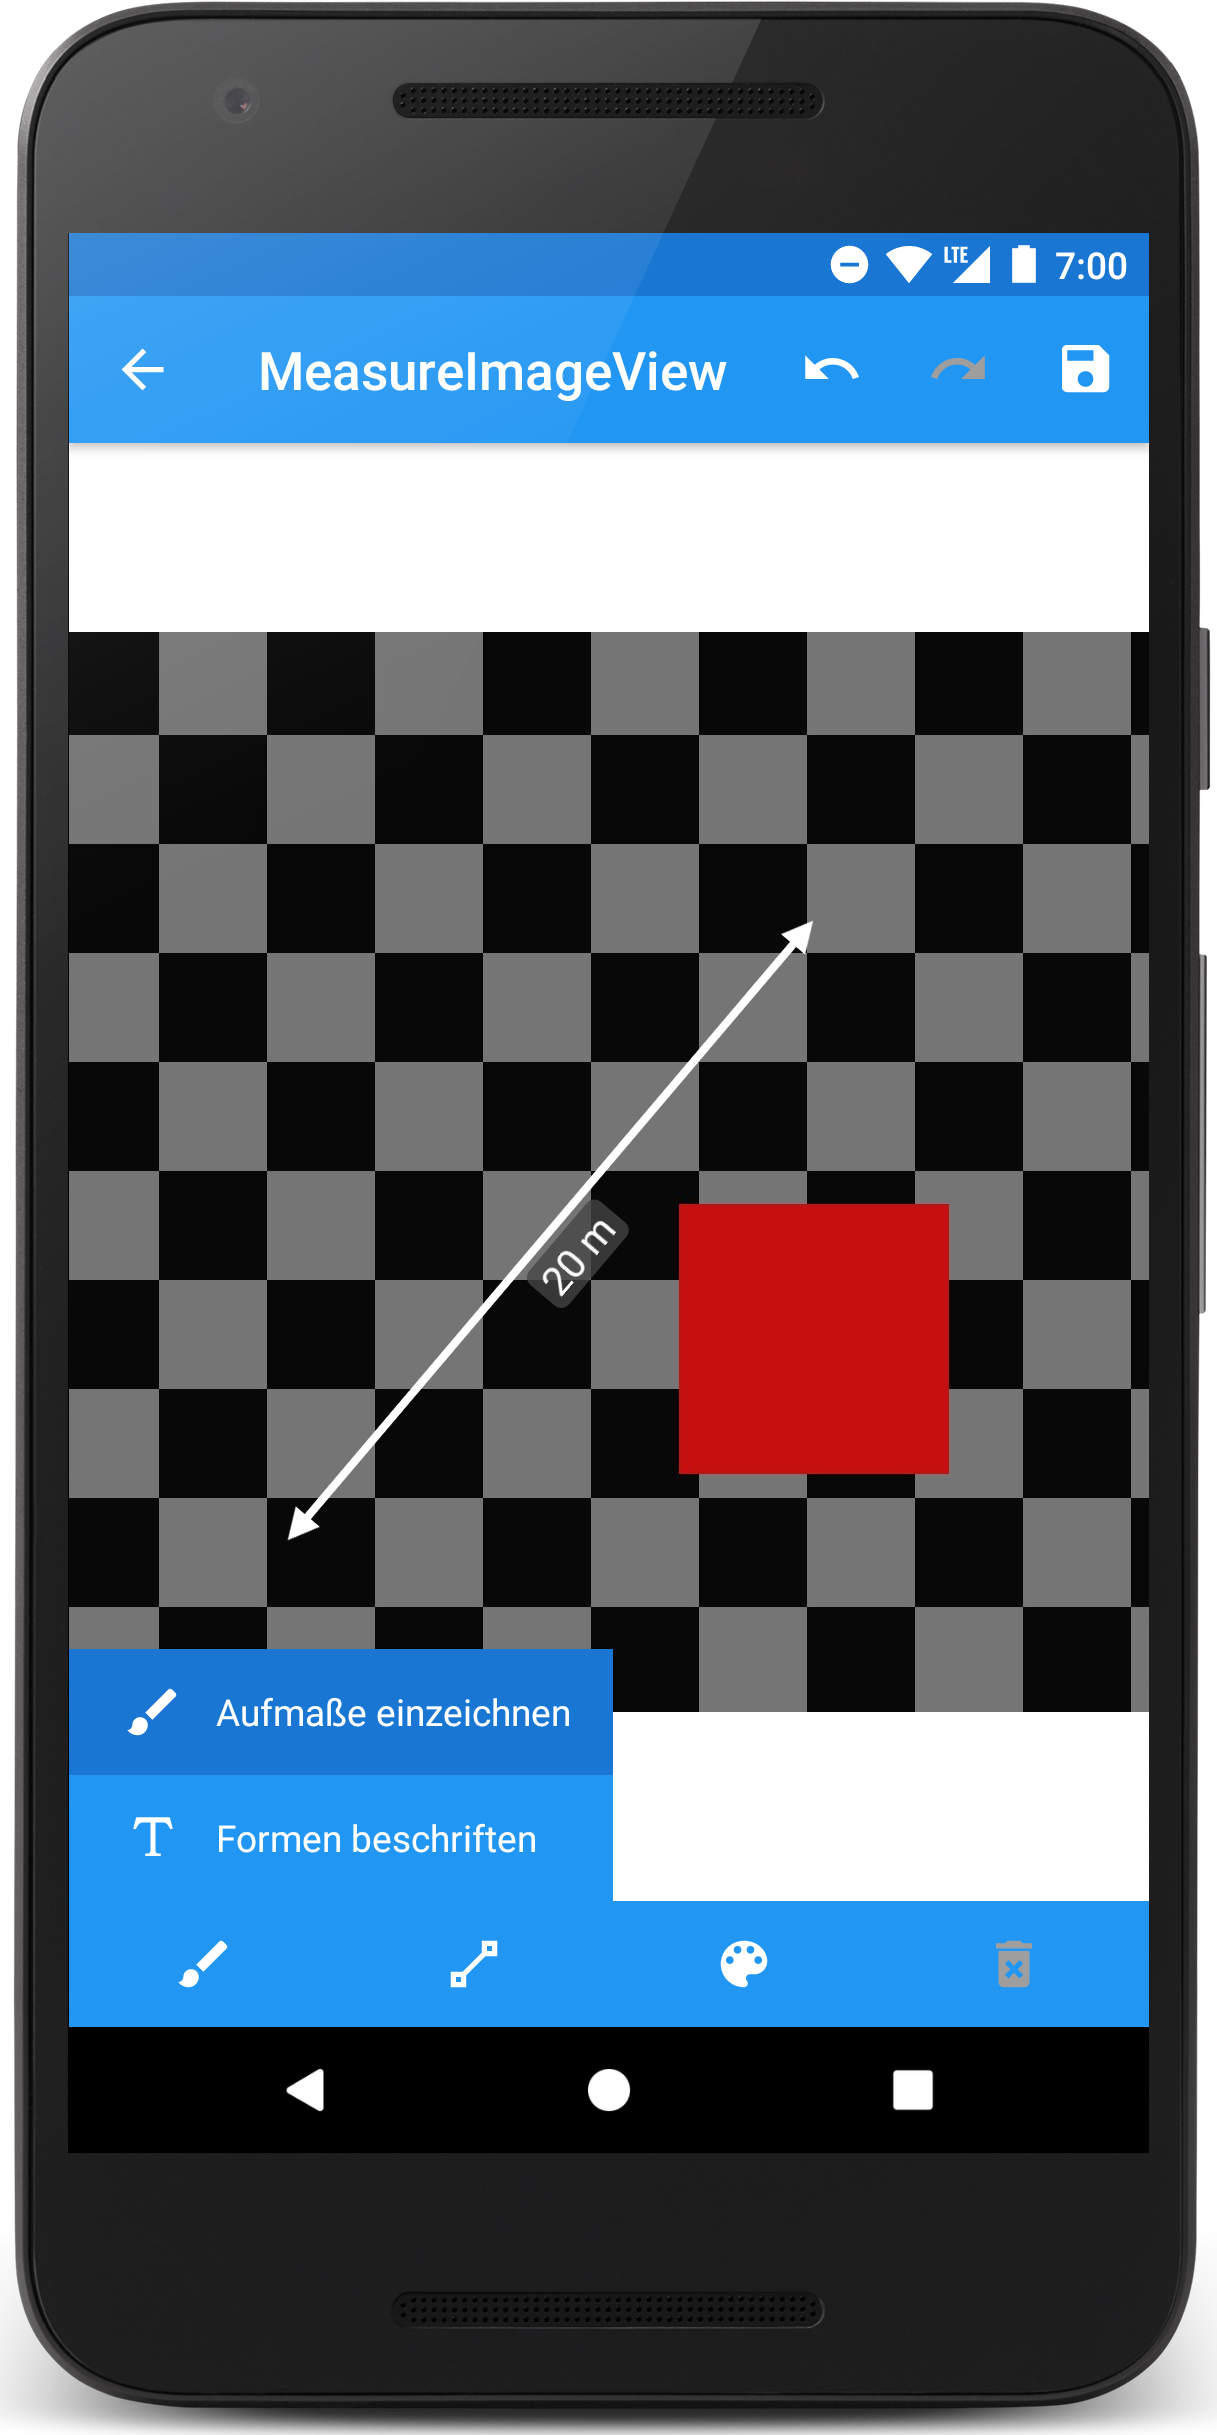
\includegraphics[keepaspectratio, width=\textwidth]{prototype2/expanded_mode}
    \caption{Statusleiste im Zeichen-Modus mit Popup-Dialog zur Auswahl des Modus}
    \label{fig:mode2}
  \end{subfigure}
  ~
  \begin{subfigure}[t]{0.4\textwidth}
    \centering
    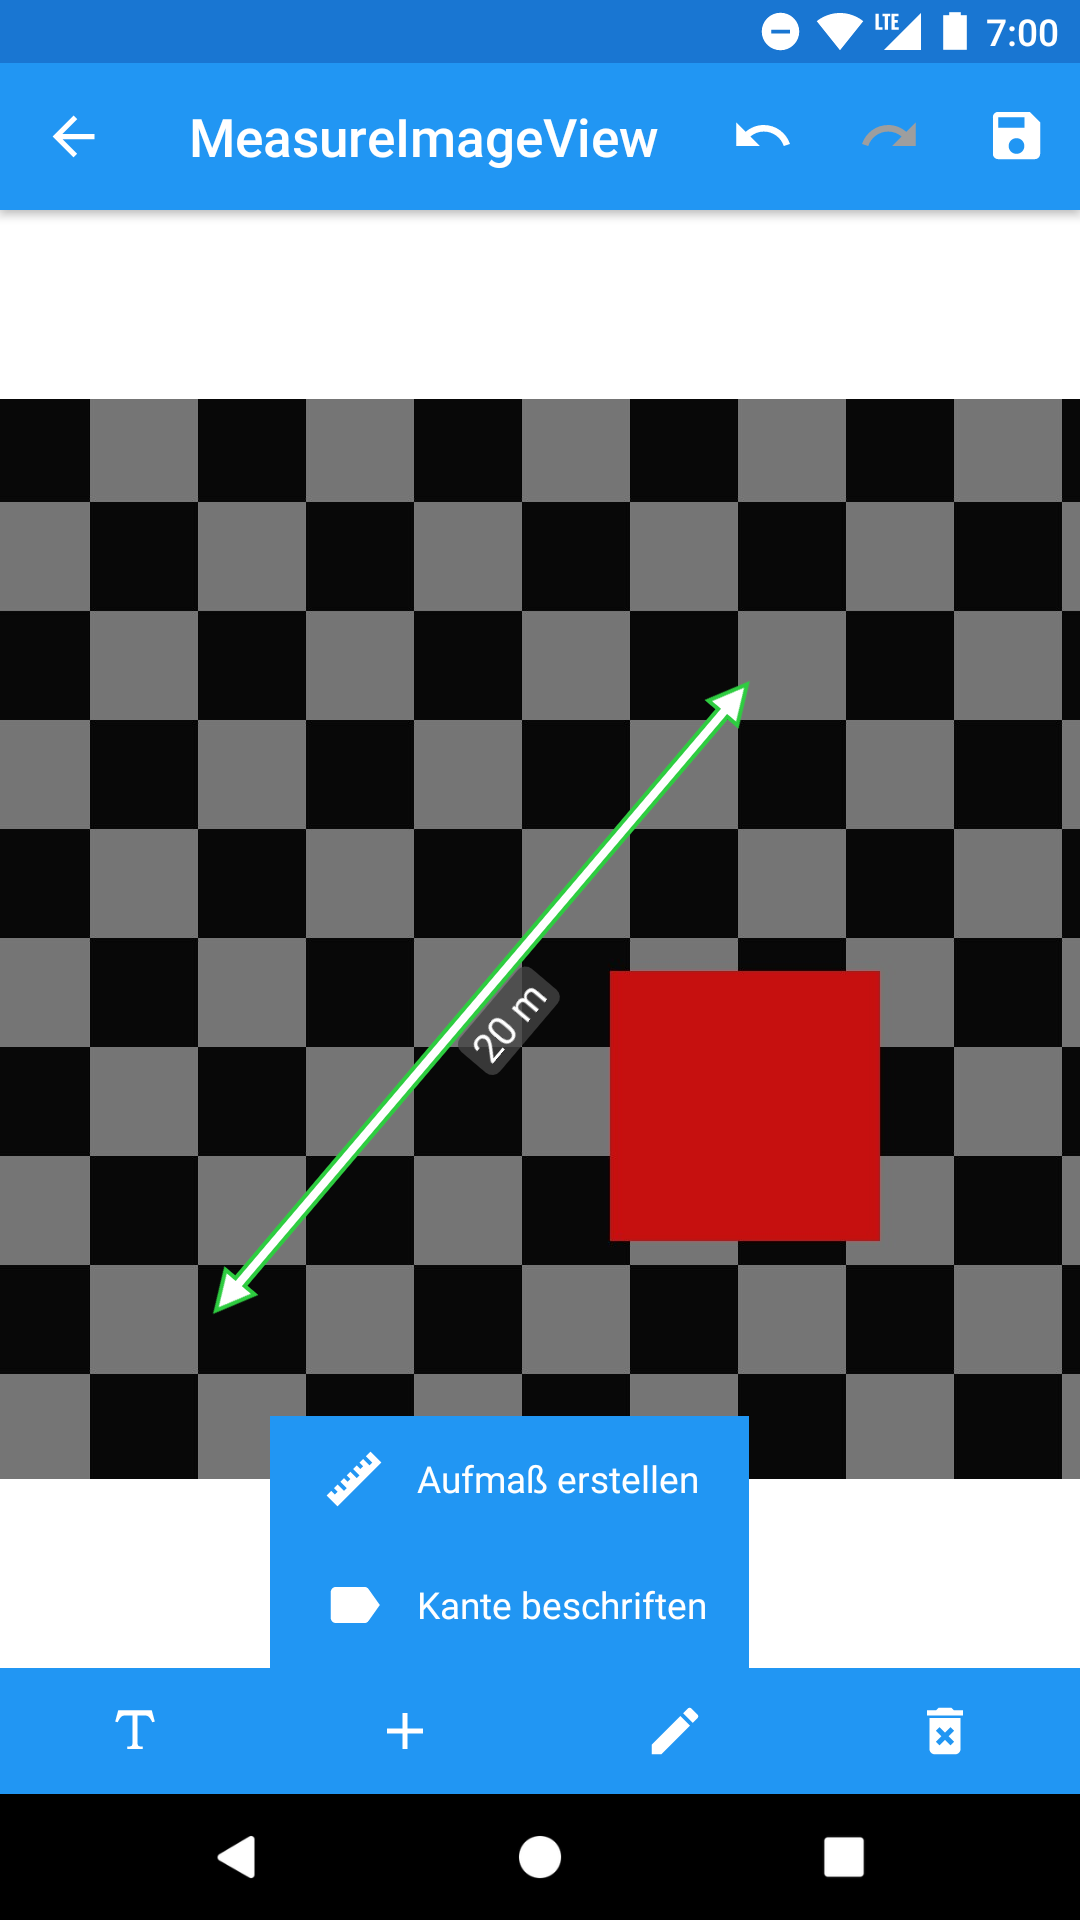
\includegraphics[keepaspectratio, width=\textwidth]{prototype2/label_popup}
    \caption{Statusleiste im Text-Modus mit Popup-Dialog zur Beschriftung der ausgewählten Form}
    \label{fig:labelp2}
  \end{subfigure}
  \centering
  \caption{Bedienung der Statusleiste im zweiten Prototyp}
  \label{fig:bar2}
\end{figure}
Diese besteht aus vier verschiedenen Icons, die nur dann auswählbar sind, wenn die entsprechende Aktion im aktuellen Systemzustand durchführbar ist.
Das Pinsel- bzw. Text-Icon ganz links in der Leiste ermöglicht das Wechseln zwischen dem Zeichen- und Text-Modus (siehe \autoref{fig:mode2}). \\

\begin{wrapfigure}{R}{0.4\textwidth}
  \centering
  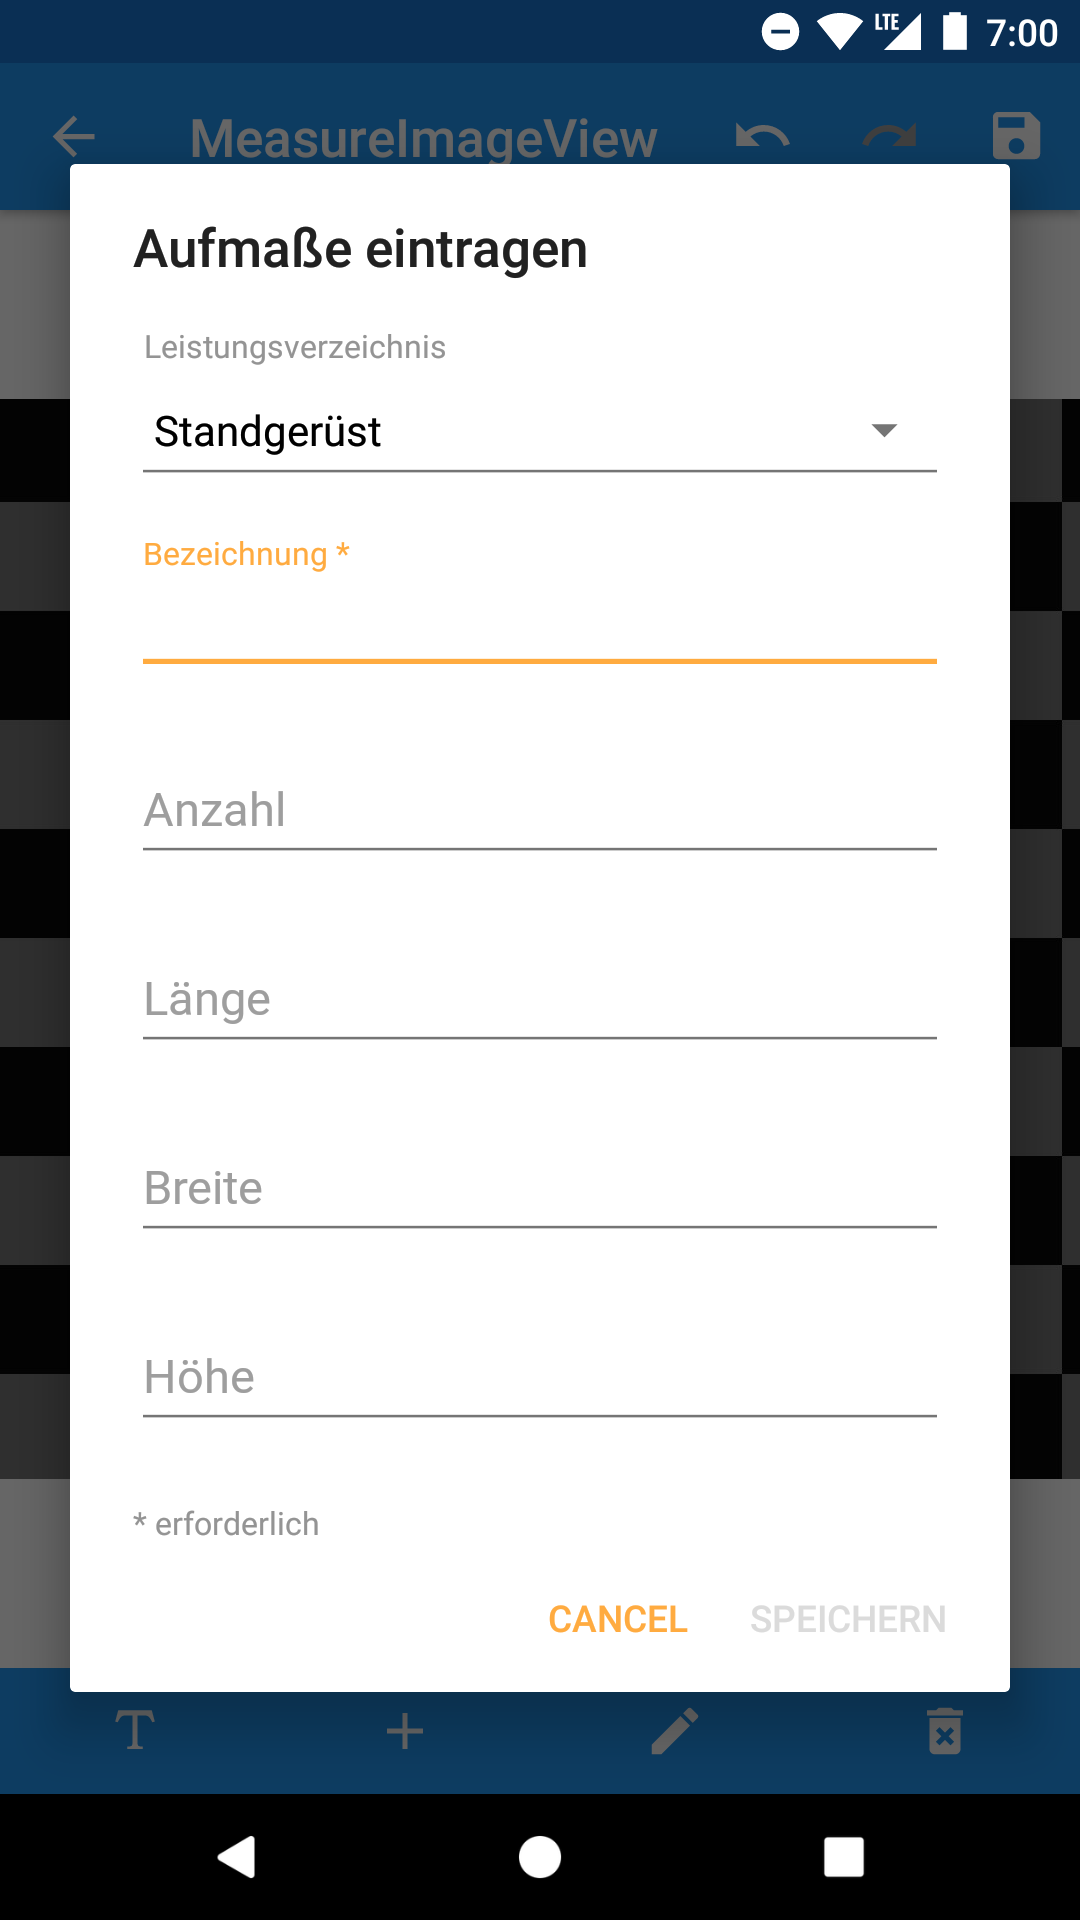
\includegraphics[keepaspectratio, width=0.4\textwidth]{prototype2/measure}
  \caption{Gerüsttyp-Dialog des zweiten Prototyps}
  \label{fig:dialog2}
\end{wrapfigure}

Im Zeichen-Modus (vgl. \autoref{fig:mode2}) kann per Klick auf das zweite Icon von links die gewünschte Form ausgewählt werden. 
Das Icon passt sich beim Ändern der Form an, und gibt so jederzeit Auskunft über die aktuell ausgewählte Zeichenform.
In \autoref{fig:mode2} ist bspw. zur Zeit die Linien-Form ausgewählt.
Im selben Modus kann beim Klick auf das dritte Icons (Farbpalette) die gewünschte Zeichenfarbe im Voraus konfiguriert werden. 
Hierzu öffnet sich, wie schon beim ersten Prototyp, ein modaler Farbauswahl-Dialog.
Auch dieses Icon passt sich dem Systemzustand an, und zeigt zu jeder Zeit die ausgewählte Farbe.
So ist in \autoref{fig:mode2} bspw. aktuell die Farbe Weiß ausgewählt.
Das vierte Icon (Mülleimer) ermöglicht im Zeichen- sowie im Text-Modus das Löschen der zuvor ausgewählten Form bzw. des markierten Textes. 
Hierbei wird der Nutzer nicht nach einer Bestätigung des Löschvorgangs gefragt, da unabsichtlich gelöschte Formen über die Undo-Funktion wiederhergestellt werden können. \\

Im Text-Modus kann beim Klick auf das zweite Icon von links (Plus-Zeichen) entweder eine ausgewählte Form mit einer Beschriftung versehen, oder mit einem Gerüsttyp verknüpft werden (siehe \autoref{fig:labelp2}).
Beim Hinzufügen einer Beschriftung öffnet sich ein modaler Eingabedialog, in den der Benutzer den gewünschten Text eintragen kann.
Entscheidet sich der Nutzer die ausgewählte Form mit einem Gerüsttyp zu verknüpfen, so öffnet sich der Gerüsttyp-Dialog (siehe \autoref{fig:dialog2}), der dem Nutzer über ein ``Dropdown'' alle möglichen Gerüsttypen zur Verfügung stellt.
Das dritte Icon von links (Stift) ermöglicht das Bearbeiten von bereits eingetragenen Messwerten und verknüpften Gerüsttypen.
Auch in diesem Modus sind die Icons nur dann auswählbar, wenn der aktuelle Systemzustand dies zulässt. 
So ist bspw. in \autoref{fig:mode2} keine Form ausgewählt, und deshalb das Mülleimer-Icon nicht auswählbar. 
In \autoref{fig:labelp2} dagegen kann die ausgewählte Linie ohne Probleme gelöscht werden. \\

Für eine einfachere und nicht so fehleranfällige Benutzung auf Tablet-Geräten wurden sämtliche Größen mit Hilfe von dichteunabhängigen Pixeln modelliert, wie sie in den ``Android Developer Guides'' suggeriert werden.
So sind hierbei alle Größen der UI-Elemente in der Einheit \emph{dp} (``density-independent pixel'') angegeben, welche zur Laufzeit vom Android-System in normale Pixel (\emph{px}) umgewandelt werden.
Die genaue Umformung lautet dabei wie folgt:
\[
  px =  dp \times (\frac{dpi}{160}),
\]
wobei $dp$ für ``dots per inch'' steht.
Dies stellt sicher, dass alle Elemente unabhängig von der Bildschirmgröße gleich groß dargestellt werden. \\

Um die Lesbarkeit der eingetragenen Messwerte bei dunkleren Bildern zu verbessern, wurde die Textfarbe der Messwerte auf weiß geändert und zusätzlich wurden halbtransparente schwarze Rechtecke hinter den Text gelegt (siehe \autoref{fig:label2}).
Hierdurch soll vermieden werden, dass der Text auf dunkleren Bildern, wie bspw. in \autoref{fig:label1}, nicht gut lesbar ist.
\begin{figure}[h]
  \begin{subfigure}[t]{0.4\textwidth}
    \centering
    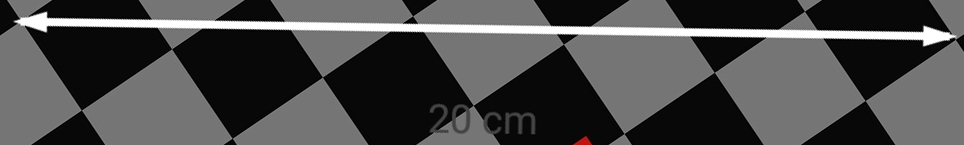
\includegraphics[keepaspectratio, width=\textwidth]{prototype2/label1}
    \caption{Eingetragener Messwert beim ersten Protoyp}
    \label{fig:label1}
  \end{subfigure}
  ~
  \begin{subfigure}[t]{0.4\textwidth}
    \centering
    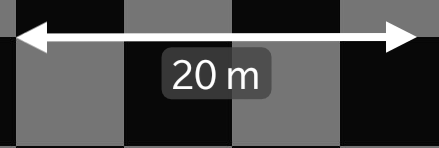
\includegraphics[keepaspectratio, width=\textwidth]{prototype2/label2}
    \caption{Eingetragener Messwert beim zweiten Prototyp}
    \label{fig:label2}
  \end{subfigure}
  \centering
  \caption{Vorher-Nachher-Vergleich: Darstellung der eingetragenen Messwerten}
  \label{fig:labels}
\end{figure}

Das Zuordnen von Gerüsttypen zu gezeichneten Formen wurde mit Hilfe eines modalen Dialogs umgesetzt, der neben dem Gerüsttyp auch noch Textfelder für die verschiedenen Dimensionen des Gerüsts besitzt.
Hierdurch kann der Benutzer nicht nur den Gerüsttyp, sondern auch Maße des Gerüsts, welche im Bild aufgrund des Aufnahmewinkels eventuell nicht zu sehen sind, eintragen und in den Meta-Daten speichern.
Verknüpfte Formen zeigen mittels eines Indikators, ob und mit wie vielen Gerüsttypen sie verbunden sind.
Auf diese Weise soll der Benutzer die bereits verknüpften von den nicht-verknüpften Formen unterscheiden können. \\

Für das Schneiden und Rotieren von Bildern vor dem Annotieren wurde \emph{uCrop}\urlnote{https://github.com/Yalantis/uCrop}, eine dedizierte Android-Library, in das Projekt eingebunden.
\emph{uCrop} ist auf \emph{Github} als \emph{Open-Source} Projekt verfügbar und kann so den eigenen Bedürfnissen angepasst werden. 
Zudem unterstützt \emph{uCrop} alle Android-Geräte unabhängig vom Gerätehersteller ab der Android-Version \emph{Ice Cream Sandwich}. 
Dies entspricht laut der Verteilung der Android-Versionen auf allen Geräten mit Android OS im Zeitraum vom 5. bis 11. Dezember 2017 mehr als $99\%$ aller Geräte (vgl. \autoref{fig:versionchart}).
Zusätzlich zum Zuschneiden und Rotieren des Bildes bietet \emph{uCrop} auch das Ändern des Bildformates an (siehe \autoref{fig:ucrop}).
Hier kann der Nutzer auswählen, ob das Bild im originalen, ``1:1'', ``3:4'', ``3:2'' oder ``16:9'' Bildseitenverhältnis importiert werden soll.

\begin{figure}[h]
  \begin{subfigure}[t]{0.4\textwidth}
    \centering
    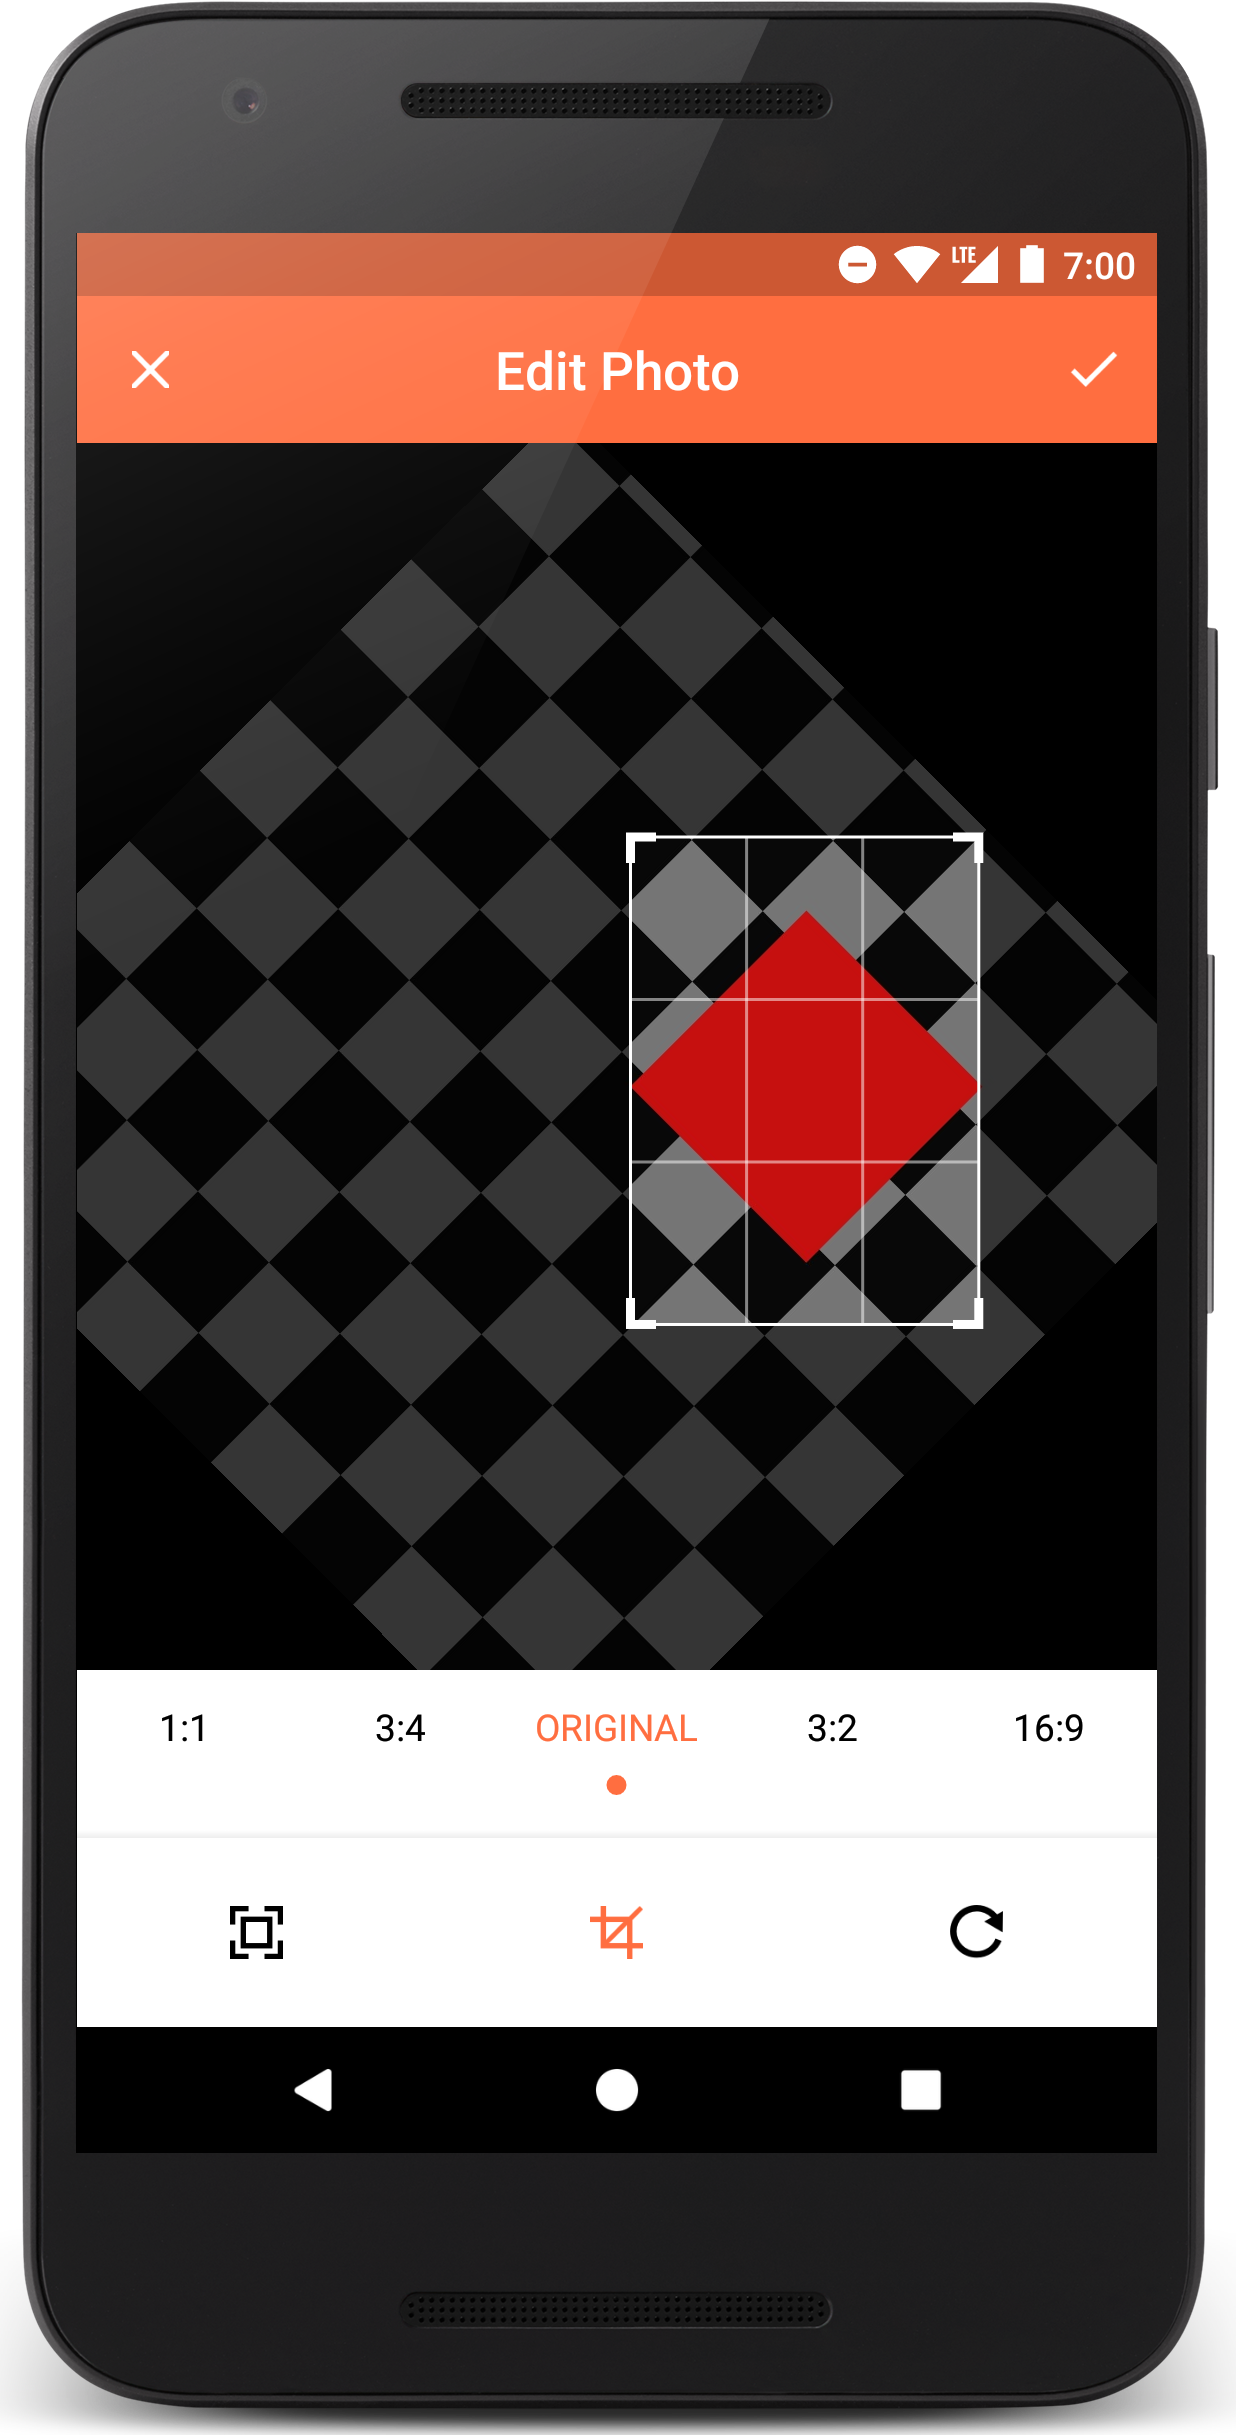
\includegraphics[keepaspectratio, width=\textwidth]{prototype2/ucrop}
    \caption{Rotation und Verkleinerung des Bildbereichs}
  \end{subfigure}
  ~
  \begin{subfigure}[t]{0.4\textwidth}
    \centering
    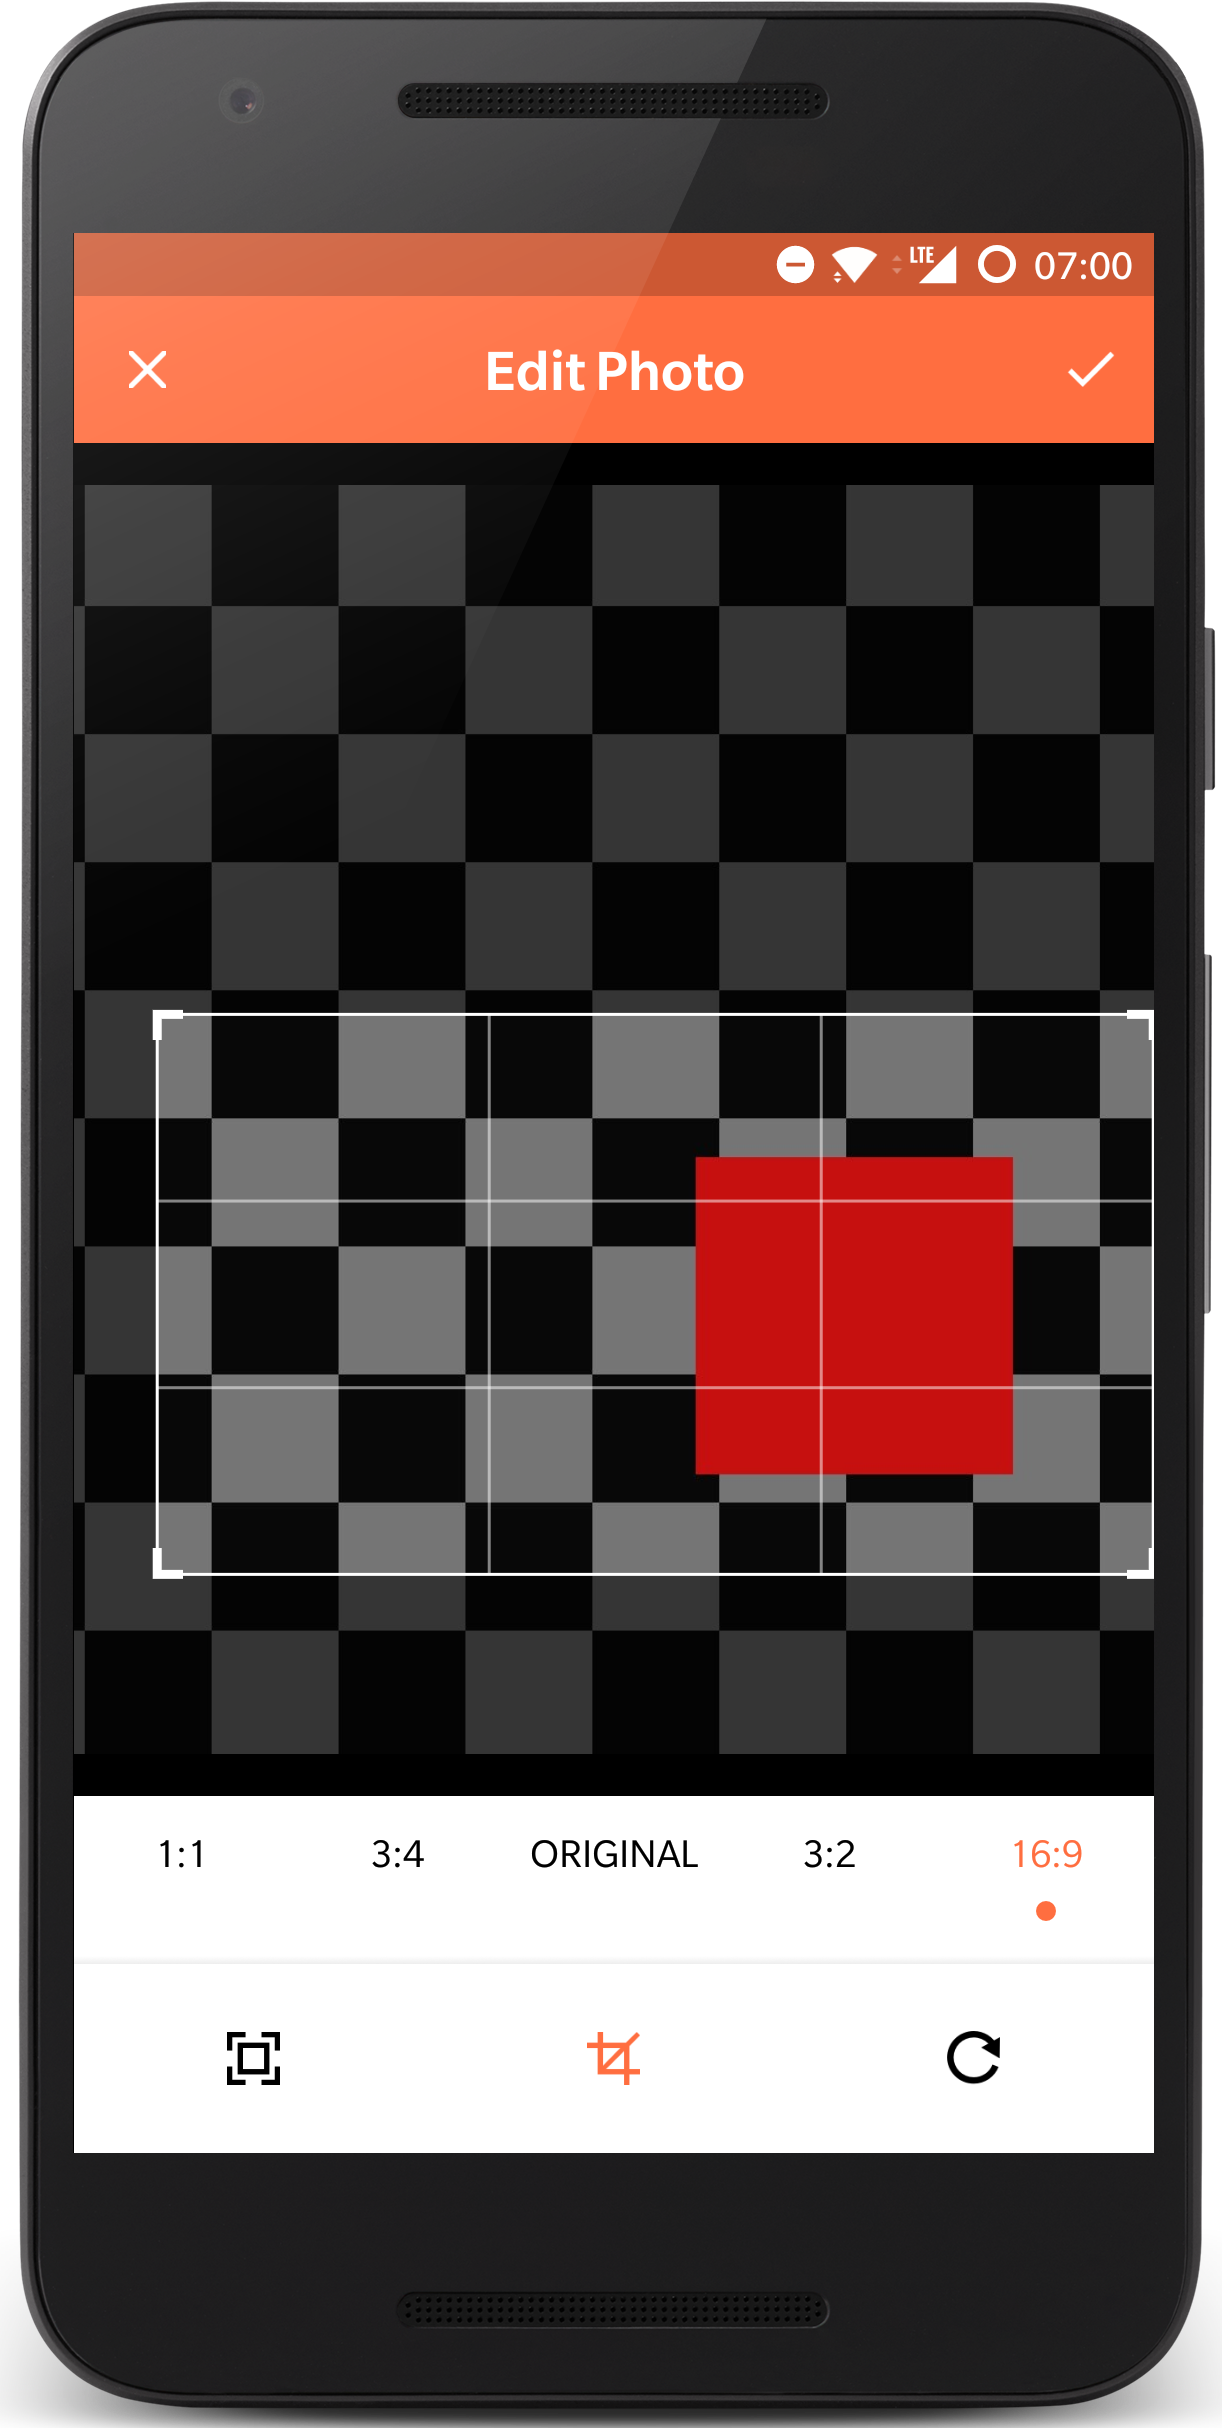
\includegraphics[keepaspectratio, width=\textwidth]{prototype2/ucrop2}
    \caption{Änderung des Bildseitenverhältnis auf ``16:9''}
  \end{subfigure}
  \centering
  \caption{\emph{uCrop}-Library zum Zuschneiden des Bildes im zweiten Prototyp}
  \label{fig:ucrop}
\end{figure}

\section{Testing}\label{sec:test2}
Der zweite Prototyp wurde sechs Tage, vom 3. bis zum 9. Januar 2018, von den beiden Testpersonen in ihren Arbeitsalltag integriert.
Das anschließende Feedback resultiert aus einem Gespräch mit beiden Testpersonen am 9. Januar. \\

Als deutlich positive Verbesserung wurde dabei von beiden Testpersonen die neue Statusleiste am unteren Bildschirmrand genannt.
Hierdurch sei ihnen die Benutzung der App um einiges leichter gefallen, als noch beim ersten Prototyp mit den \emph{Floating Action Buttons}. \\

Jedoch sei, so beide Tester, das initiale Einarbeiten in die App immer noch zu schwierig, und nicht intuitiv genug.
Hier wünsche man sich eine ``kleine Anleitung, die die App kurz beschreibt'' (Testperson 2) \\

Ein weiteres Problem, dass beim Testen des Prototyps aufgefallen ist, sei der Farbdialog.
Dieser sei nach Aussage von Testperson 1, zu fortgeschritten und biete eine Auswahl an Farben, die ``[...] der normale Gerüstbauer niemals verwenden wird'' (Testperson 1).
Hierbei wäre es laut Testperson 1 sinnvoller, den Benutzer ``[...] nicht mit so vielen Auswahlmöglichkeiten zu überschütten [...]'', sondern die populärsten Farben direkt auswählbar zu machen. \\

Außerdem wurde sich neben einem einfacheren Farbdialog eine Funktion gewünscht, Freitexte in das Bild eintragen zu können. 
Dies sei laut der Aussage beider Tester eine wichtige Funktion, da es bisher keine Möglichkeit gibt, weitere Notizen oder Anmerkungen im Bild zu hinterlegen \\

Zudem kam der Wunsch nach einer weiteren Form, nämlich einer Linien mit nur einer Pfeilspitze, auf.
Dies sei, so beide Testpersonen, wichtig, um Längen, die auf dem Bild nur einen Startpunkt haben, und in die Tiefe offen sind, zu kennzeichnen oder bestimmte Details hervorzuheben. \\

Des Weiteren seien verlinkte Gerüsttypen an Formen nicht intuitiv durch den in diesem Prototyp eingeführten Indikator erkennbar.
Hierzu fügten beide Testpersonen hinzu, dass die Eingabefelder zum Eintragen der Messwerte im Gerüsttyp-Dialog ``[...] durchaus sinnvoll [...]'' (Testperson 1) seien, in der Praxis jedoch daran scheitern würde, dass sich Messwerte zuerst gemerkt werden müssen, bevor sie im Dialog eingegeben werden können.
Dies habe sich besonders dann als Problem herausgestellt, wenn mehr als ein Messwerte zugleich eingetragen werden sollten. \\

Zusammenfassend lässt sich festhalten, dass sich in dieser Testphase sowohl neue Usability-Probleme, als auch neue Anwenderwünsche identifizieren lassen haben.
Diese Ergebnisse sollen in einer weiteren Iteration des \hcdp{} im nächsten Kapitel genauer untersucht werden.
